\documentclass[journal]{IEEEtai}

\usepackage[colorlinks,urlcolor=blue,linkcolor=blue,citecolor=blue]{hyperref}

\usepackage{color,array}

\usepackage{graphicx}

\usepackage{soul}

\usepackage{makecell}
\usepackage{graphicx}
\usepackage{textcomp}
\usepackage{array} 
\usepackage{longtable}
\usepackage{booktabs}
\usepackage{float}
\usepackage{subcaption}
\usepackage{amsmath}
%% \jvol{XX}
%% \jnum{XX}
%% \paper{1234567}
%% \pubyear{2020}
%% \publisheddate{xxxx 00, 0000}
%% \currentdate{xxxx 00, 0000}
%% \doiinfo{TQE.2020.Doi Number}

\newtheorem{theorem}{Theorem}
\newtheorem{lemma}{Lemma}
\setcounter{page}{1}
%% \setcounter{secnumdepth}{0}


\begin{document}


\title{INT104 CW3-Lab report} 


\author{Ruiyang.Wu\quad	sID:2257475\quad E-Mail:Ruiyang.Wu22@student.xjtlu.edu.cn
	\\
	TA: Yu Kang \quad E-Mail:Yu.kang23@student.xjtlu.edu.cn
}

\markboth{INT104 Artificial Intelligence CW3 2024/05/24 Ruiyang.Wu}
{INT104 Artificial Intelligence CW3 2024/05/24 Ruiyang.Wu}

\maketitle


\section{\textbf{Introduction}}

\IEEEPARstart{I}{n} this experiment, I firstly used Gaussian Mixture Model (GMM), k-means and hierarchical clustering to fit the clusters to the samples in the Treated Sample Space, optimised the clustering hyper-parameters using Grid Search and evaluated the clustering results using Adjusted Rand Index (ARI). After obtaining better clustering results, the distribution of samples in each cluster is then examined. I use this to assess the association of the clustered clusters with the Programmes in which the students are enrolled, as well as to formulate relevant scientific hypotheses. To ensure the re-implementation of the experiments, the relevant results and code are saved in the following repository:
\href{https://github.com/MushihimePepsi/XJTLU_ICS_Y2S2_Course-notes_23-24/tree/main/INT104-%E4%BA%BA%E5%B7%A5%E6%99%BA%E8%83%BD}{\ul{https://github.com/MushihimePepsi/XJTLU\_ICS\_Y2S2\\\_Course-notes\_23-24/tree/main}}


\section{\textbf{Before clustering: Claims on Clustering criteria, Visualizations \& Input features}}
\subsection{\textbf{Consider using more than the number of labels for the clusters: Sub-populations}}
Although we tend to use the number equivalent to the sample category as the number of clusters for clustering algorithms, with a hope of obtaining clusters that can correspond one-to-one with the true category of the sample. However, in the actual sample space, there may be more refined sub-populations of samples of the same category with different feature distributions. For example, if there are 4 labels representing 4 types of fruits, but there are several different varieties of each fruit, using more clusters than the number of labels may identify these varieties separately and at the end assign each cluster to the most frequent category label using Majority Voting, or using the Hungarian algorithm's Cost of Assignment Minimization (COA) to assign each cluster to the category it belongs to. In this way, we may obtain more accurate clustering results. 

However, it is also important to note that the assessment of the clustering effect in this case should not be done using Accuracy or Rand index (RI), since these assessments increase with the number of clusters even if the labels are randomly assigned. As an alternative, we should use the ARI.

\subsection{\textbf{Selection of performance metrics for clustering}}
\subsubsection{\textbf{Why choosing ARI rather than Accuracy?}}
In previous supervised learning operations, we often used Accuracy as a metric for evaluating model performance; however, in clustering algorithms which belong to unsupervised learning, since the number of clusters may not be equal to the actual number of categories and the algorithm cannot directly determine the category labels to each cluster, the use of confusion matrices or Accuracy as a metric is inappropriate. In this case, we can choose Normalised Mutual Information (NMI) or Adjusted Rand Index (ARI) to judge the degree of matching between the clustering results and the real labels. However, as the number of clustered clusters increases, the evaluation values of Accuracy, NMI, etc. increase with the number of clusters even if labels are randomly assigned to each cluster. To punish the false performance due to random classification and category imbalance, I used ARI here, an index that takes into account the expected value of randomly assigned labels, to reflect the quality of the clustering results more reliably.

\begin{center}
	\text{\textbf{Formula of Adjusted Rand Index}}
	\begin{align} 
		ARI &= \frac{\text{RI} - \text{Expected RI}}{\max(\text{RI}) - \text{Expected RI}} \in [-1,1]
		\\ Where&:
		\left\{\begin{matrix}
			\text{RI} = \frac{a + b}{a + b + c + d}
			\\
			\text{Expected RI} = \frac{\sum_i \binom{a_i}{2} \sum_j \binom{b_j}{2}}{\binom{n}{2}}
		\end{matrix}\right.
	\end{align}
	\begin{flushleft}
	\text{\textit{a: Pairs in the same cluster in true and predicted.}}
	\text{\textit{b: Pairs in different clusters in true and predicted.}}
	\text{\textit{c: Pairs in the same cluster in true but different in predicted.}}
	\text{\textit{d: Pairs in different clusters in true but same in predicted.}}
	\text{\textit{The closer to 1 the clustering is matched to the real situation.}}
	\end{flushleft}
\end{center}

\subsubsection{\textbf{Failure of Silhouette Coefficients and Elbow Methods}}
In most cases, a cluster should have two good properties: cohesion and separation. This means that, in the usual sense, samples in the same cluster are as close as possible while being as away as possible from elements in other clusters, since the fact that we assume samples of the same class have similar feature distributions. Under the influence of this heuristic, coefficients such as Silhouette coefficient implicitly expect clusters that better reflect the true labels by judging the degree of cohesion and separation of the clusters generated by a clustering. However, in this task, the samples were extremely close in distance and density, except the students  `Programme'=3. None of the coefficients using this heuristic were effective in judging the performance of this  task.

\begin{figure}[htbp]
	\centerline{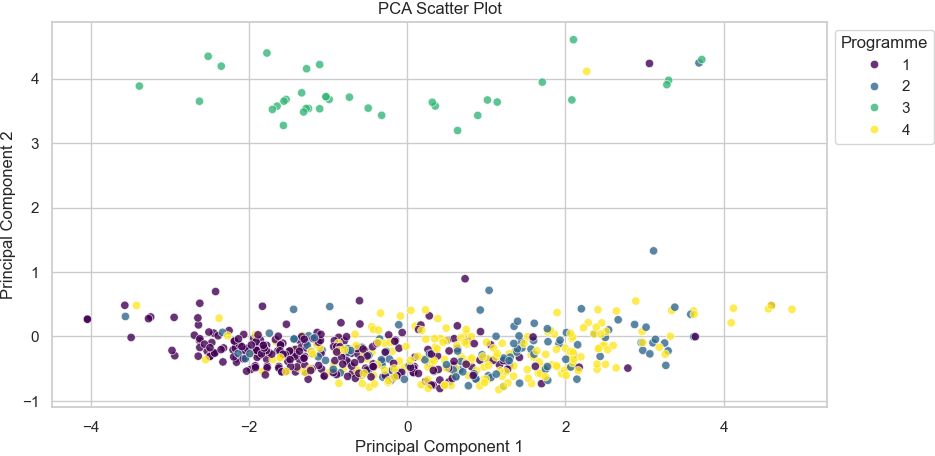
\includegraphics[width=17pc]{pca_7_features_in.png}}
	\caption{Raw data distribution: Lack of clustering tendency}
\end{figure}

\subsubsection{\textbf{The Necessity of Dividing Training and Test Sets in Unsupervised Learning}}
Although the use of dividing the training and test sets and cross-validation in some unsupervised learning tasks helps to assess the generalization ability of the model, dividing the training and test sets is not very meaningful in this task, especially when ARI has been used to assess the clustering ability. In addition, the total number of samples in this experiment is too small and faces the problem of class imbalance, which even with the use of under-sampling or Synthetic Minority Over-sampling Technique (SMOTE) results in a test set that does not fully reflect the true effect of clustering. Overall, unsupervised learning focuses more on discovering underlying structures and patterns from the data, and training with the full data tends to achieve this goal better, providing more stable and comprehensive evaluations.


\subsection{\textbf{Selection of clustering visualization and input features}}
As this experiment used distance-based clustering methods, different sizes of input features may cause the clustering algorithm to be biased towards the importance of different features. Therefore, before clustering, the input features were uniformly Z-Score normalized to eliminate the effect of data size. In this experiment, in order to facilitate the study of the impact of different features on the clustering results, the input features were used from the original feature set, and no data from Locally Linear Embedding (LLE) or Principal Component Analysis (PCA) were used. For visualization, I used PCA to reduce the dimensional and simply used the two directions with the highest variance as the X and Y axes.

\section{\textbf{Task1: Gaussian Mixture Model}}
The correctness of the Gaussian Mixture Model comes from the assumption that the data is composed of multiple Gaussian distributions, where each Gaussian distribution acts as a cluster (component) with its own mean vector and covariance matrix. I manipulated the state of each cluster's covariance matrix by adjusting the hyper-parameter `covariance\_type' and found that in \{`full', `tied', `diag'\}, `diag' has the best clustering result ARI$\approx$ 0.17. Which means the covariance matrix is diagonal. This is the same conclusion found in cw1\&2, i.e., the contribution of each feature to the clustering is relatively independent. Only a small linear correlation between the features, while the distribution of different features is different.

\begin{figure}[htbp]
	\centerline{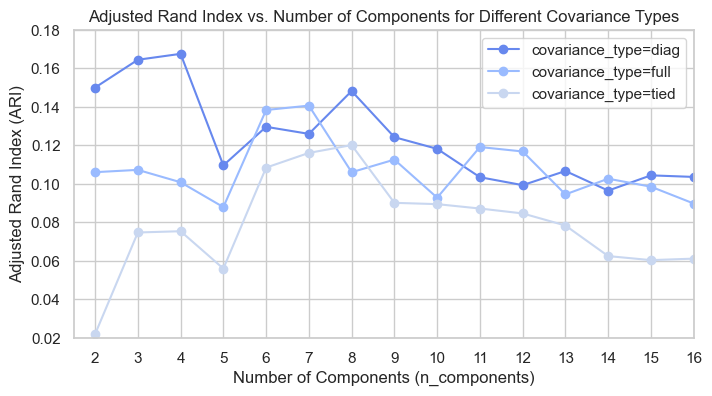
\includegraphics[width=20pc]{ARI_vs_Conv_type.png}}
	\caption{Different `covariance\_type' on clustering performance}
\end{figure}

Following through the grid search, I use the best hyperparameters to get a visualisation of the clusters with the distributions in each cluster.

\begin{figure}[htbp]
	\centerline{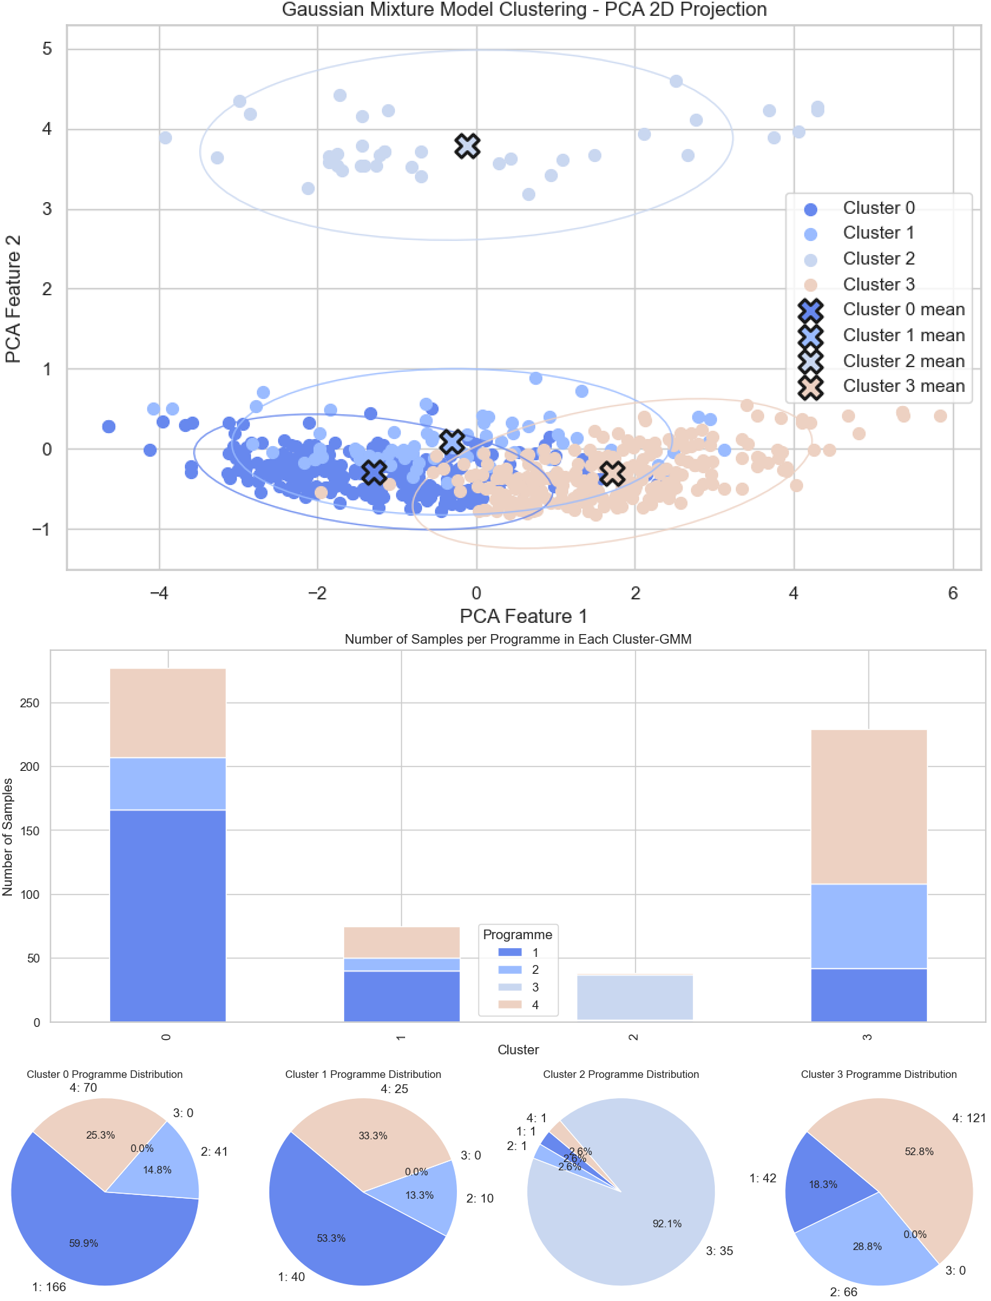
\includegraphics[width=18.3pc]{GMM-sum2.png}}
	\caption{GMM Clustering Visualization and Statistics}
\end{figure}

\section{\textbf{Task2: K-means}}
K-means is a distance-based clustering method that obtains the final cluster by assigning each point to the nearest cluster center and iterating to obtain the final cluster. For this experiment I used Euclidean distance as the distance definition for clustering and the optimization objective was to minimize Sum of Squared Errors (SSE) until convergence. Given that this method is sensitive to the choice of initial state, I used the k-means++ method to initialize the clustering centers to make the initial points more dispersed.

The highest ARI$\approx$ 0.22 is taken at n=3, but this is due to class imbalance of too few students with `Programme'=2. The clustering abandons the assignment to this class.
\begin{figure}[htbp]
	\centerline{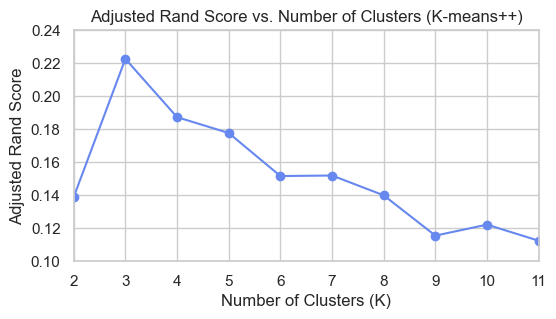
\includegraphics[width=18pc]{ARI_vs_k_k-means.png}}
	\caption{Effect of clusters number k on clustering performance}
\end{figure}

\begin{figure}[htbp]
	\centerline{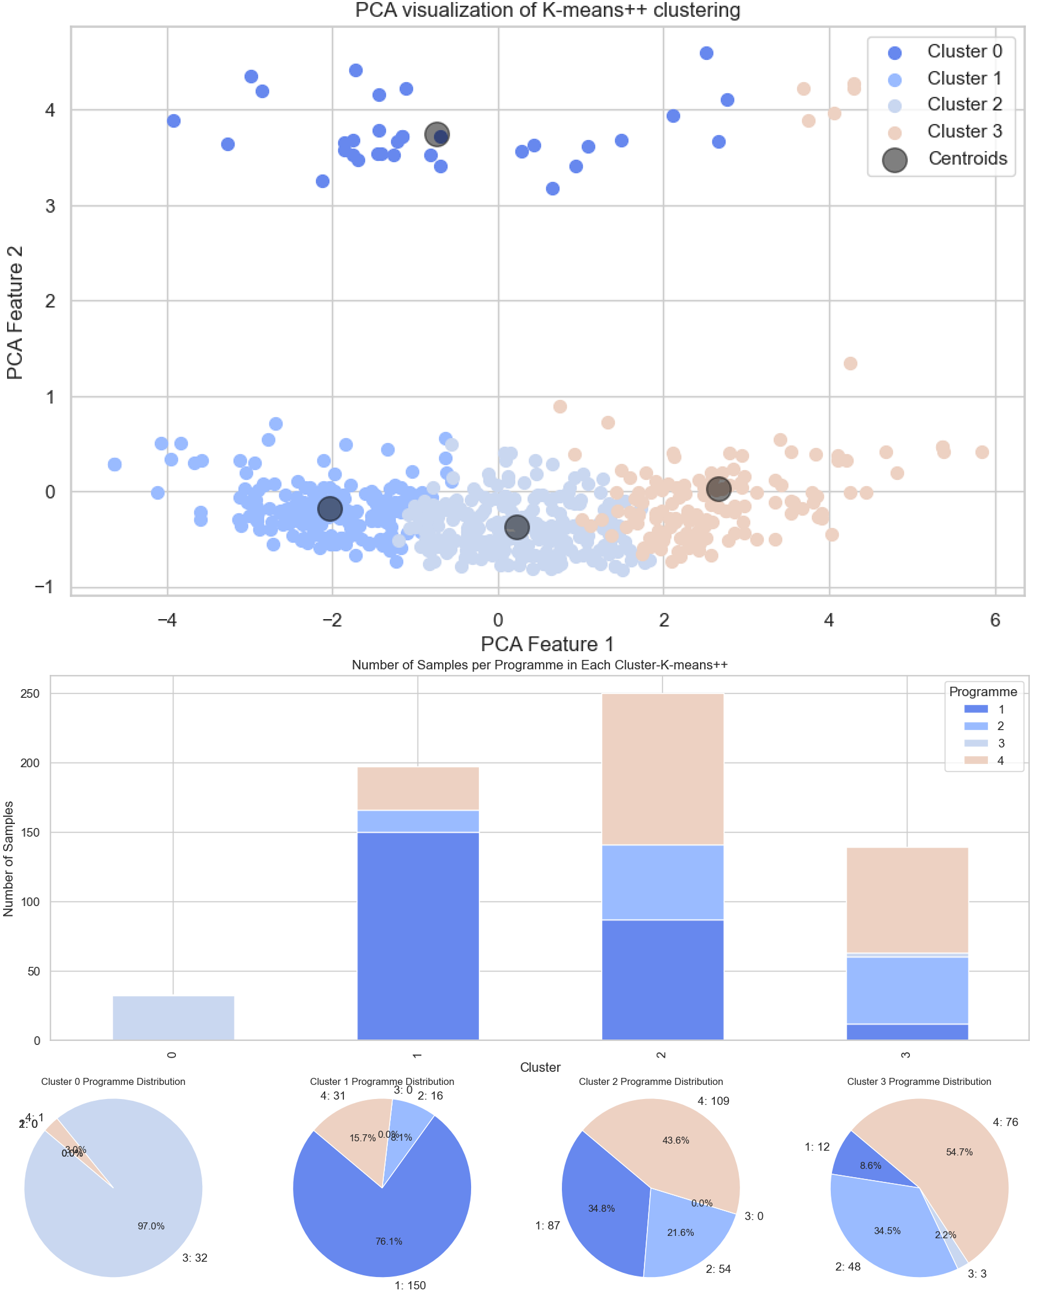
\includegraphics[width=18pc]{k-means-sum.png}}
	\caption{k-means Clustering Visualization and Statistics}
\end{figure}

\section{\textbf{Task3: Hierarchical Clustering}}
In this experiment, I used agglomerative hierarchical clustering, which is from bottom to up. It is also a distance-based clustering method that generates a clustering tree by progressively merging clusters, thus allowing for the generation of clustering results at different levels of granularity.

\begin{figure}[htbp]
	\centerline{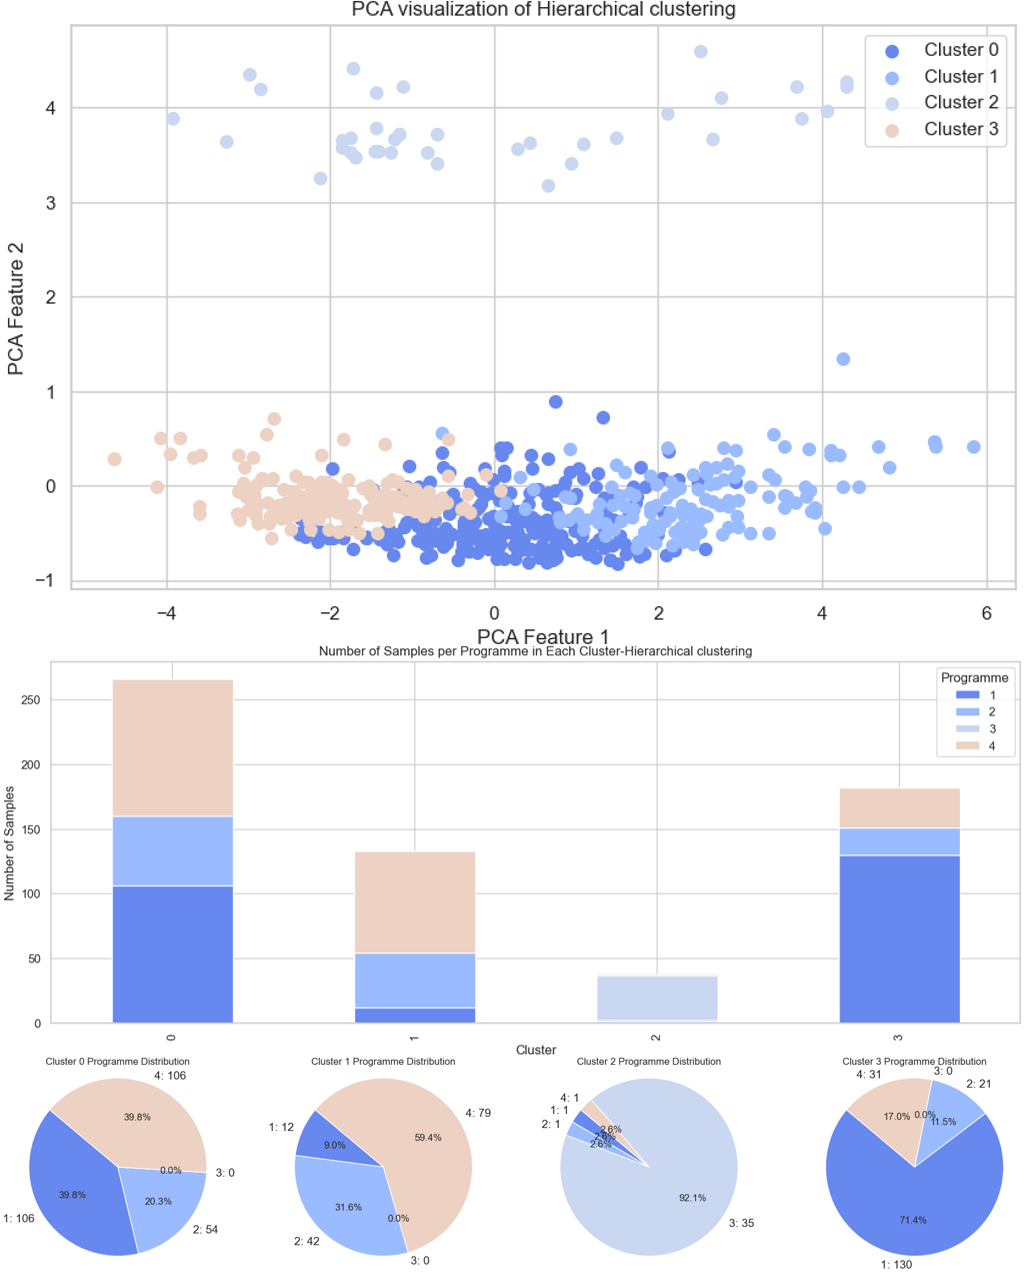
\includegraphics[width=18pc]{Hiera-sum.png}}
	\caption{k-means Clustering Visualization and Statistics}
\end{figure}

\begin{figure}[htbp]
	\centerline{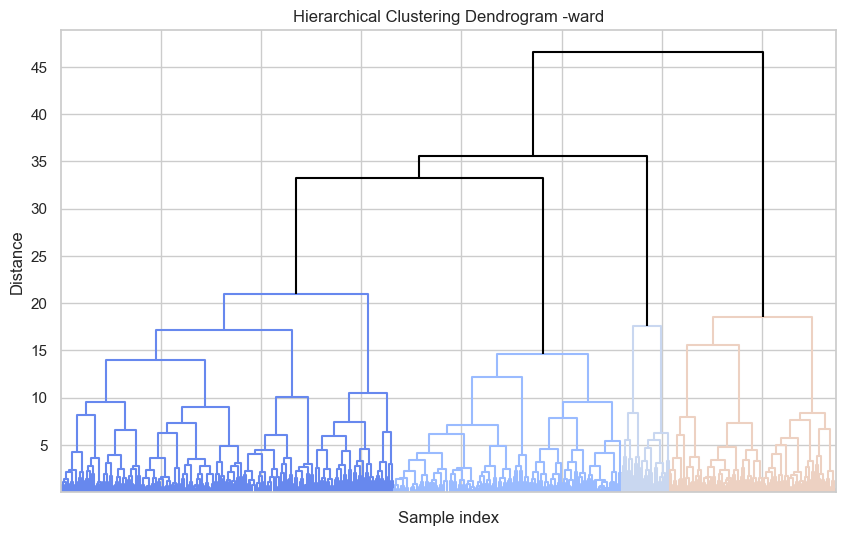
\includegraphics[width=17pc]{Hierarchical Clustering Dendrogram -ward.png}}
	\caption{Hierarchical Clustering Dendrogram: Distance=21}
\end{figure}

By adjusting the definition of distance, I found that `ward' performed best ARI$\approx$ 0.15. The increase in performance of `average' when n$\textgreater$8 is due to the imbalanced categories in the data set, and this clustering abandons the classification of samples with `Programme'=2.

\begin{figure}[htbp]
	\centerline{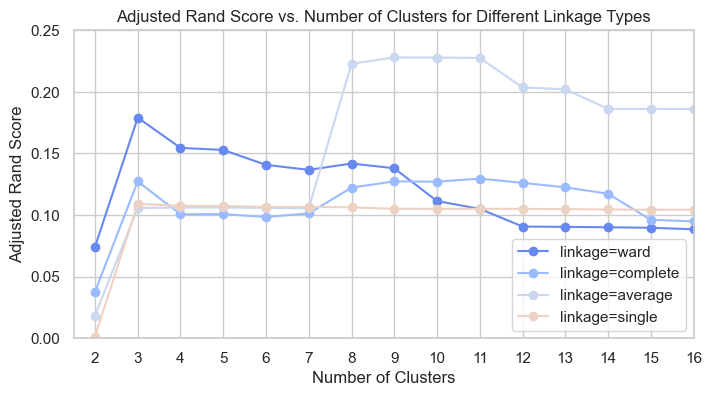
\includegraphics[width=17pc]{Different Linkage Types.png}}
	\caption{The impact of different Linkage Types on performance}
\end{figure}

\section{\textbf{Task4: Association between Clusters \& Programme}}
\subsection{\textbf{Conclusion \& Scientific hypothesis}}
The clustering methods revealed that only samples with `Programme'=3, characterized by `Grade'=3, were accurately clustered. The other samples, which exhibit a little linear relationship within the dataset, were not as precisely classified. Samples with `Programme'=2 and 4 showed no significant distributional differences, whereas samples with `Programme'=1 showed a slight tendency to be cohesive.
\subsection{\textbf{Limitations}}
In this experiment, only normalized raw features were used, and clustering algorithms based on distance or density did not capture the correlation between non-linear features or newly generated features from non-linear combinations. Future work should consider clustering features obtained through nonlinear manifold analysis or using Self-Organizing Maps (SOM) to explore deeper relationships between non-linear feature combinations and sample categories.

\section{\textbf{Acknowledgment}}
I would like to thank the two TAs of SC375: Yu Kang and Yiqiang Cai for their detailed comments and guidance, Dr. Shengchen Li for his careful design of the experiments.

\end{document}
